\section{Experimental Results and Analysis}
\label{sec:results_analysis}

\subsection{Datasets and Experimental Settings}

\begin{figure*}[!t]
  \centering
  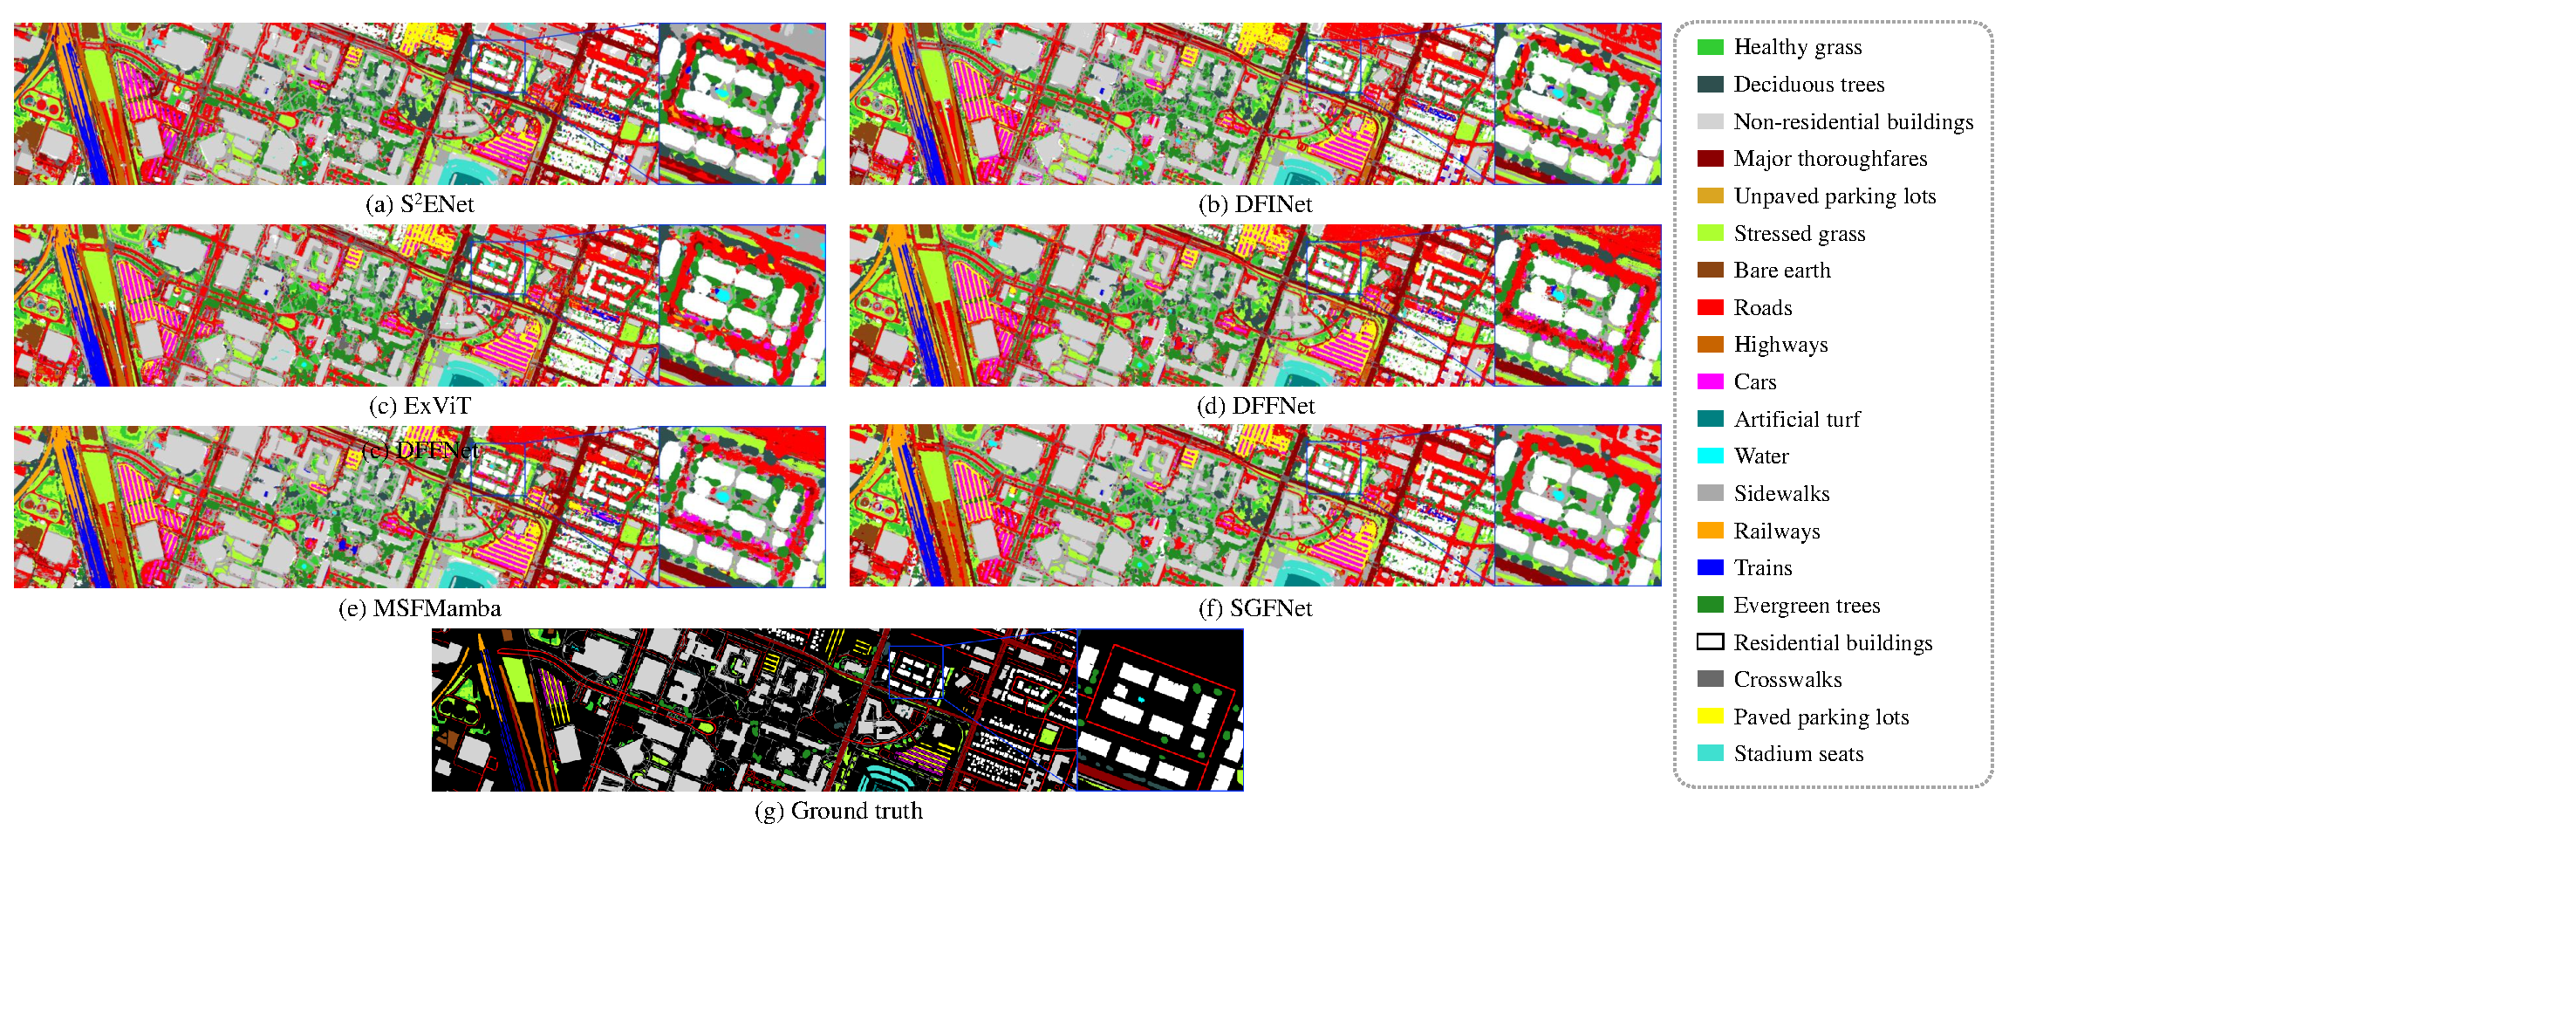
\includegraphics[width=0.8\textwidth]{figures/fig_results.pdf}
  \caption{Classification results of different methods on the Houston2018 dataset.}
  \label{fig_results}
\end{figure*}

\begin{table}
  \centering
  \caption{Experimental results on the Augsburg dataset. The \textbf{bold} and \underline{underline} denote the best and second results.}
  \setlength{\tabcolsep}{3pt} 
  \resizebox{0.90\linewidth}{!}{
  \begin{tabular}{c|ccccccc}
  \hline\toprule
  Class            & S$^2$ENet & DFINet & ExViT & DFFNet & MSFM & \cellcolor{bg}SGFNet \\
  \midrule
  Forest           & \textbf{98.10} & \underline{97.38} & 90.04 & 96.17 & 97.17 & \cellcolor{bg}97.18 \\
  Residential area & \textbf{99.08} & \underline{98.37} & 95.44 & 96.64 & 98.15 & \cellcolor{bg}98.28 \\
  Industrial area  & 12.19 & \underline{61.31} & 34.58 & 37.70 & 50.26 & \cellcolor{bg}\textbf{61.41} \\
  Low plants       & 91.78 & 92.63 & 90.68 & 94.21 & \textbf{95.52} & \cellcolor{bg}\underline{95.48} \\
  Allotment        & 45.12 & 49.33 & 51.82 & \underline{53.54} & 53.35 & \cellcolor{bg}\textbf{65.01} \\
  Commercial area  & 1.22  & 3.54  & \textbf{28.63} & \underline{11.36} & 2.63 & \cellcolor{bg}8.55 \\
  Water            & 24.09 & 26.61 & 17.65 & 27.15 & \underline{49.97} & \cellcolor{bg}\textbf{56.62} \\
  \midrule
  OA               & 88.22 & 90.66 & 86.65 & 89.37 & \underline{91.38} & \cellcolor{bg}\textbf{92.38} \\
  AA               & 53.08 & 61.31 & 58.41 & 59.54 & \underline{63.31} & \cellcolor{bg}\textbf{68.93} \\
  Kappa            & 86.47 & 86.47 & 80.79 & 84.51 & \underline{87.45} & \cellcolor{bg}\textbf{89.05} \\
  \bottomrule\hline
  \end{tabular}}
  \label{table_augsburg}
\end{table}

The performance of the proposed SGFNet is evaluated on two benchmark multi-source remote sensing datasets for land-cover classification. The first dataset is the Augsburg Dataset \cite{aug23data}, which consists of HSI and SAR data. It contains ground-truth annotations for seven land-cover classes and has a spatial size of 332 $\times$ 485 pixels. The second dataset is the Houston 2018 Dataset, which comprises HSI and LiDAR data. As it is obtained from the IEEE GRSS Data Fusion Contest 2018 \cite{xyh18grss}, this dataset provides a representative multi-sensor optical geospatial benchmark for challenging urban land-cover and land-use classification tasks over the University of Houston campus and its surrounding areas. The dataset includes hyperspectral imagery with 48 spectral bands spanning wavelengths from 380-1050 nm, along with LiDAR measurements that provide accurate elevation information.

Our SGFNet was conducted on NVIDIA GeForce RTX 5080 GPU. The training phase spanned over 100 epochs. The AdamW optimizer was used with a learning rate of 0.001. The batch size was set to 32. To evaluate the performance of the proposed SGFNet, we compare it against other state-of-the-art methods, including S$^2$ENet \cite{fs22grsl}, DFINet \cite{gyh22tgrs}, ExViT \cite{exvit}, DFFNet \cite{dffnet}, and MSFM \cite{gao2025msfmamba}. To quantitatively evaluate the experimental results, we employ three standard metrics: Overall Accuracy (OA), Average Accuracy (AA), and Kappa coefficient. 

\subsection{Parameter Analysis}

\begin{figure}[htb]
\centering
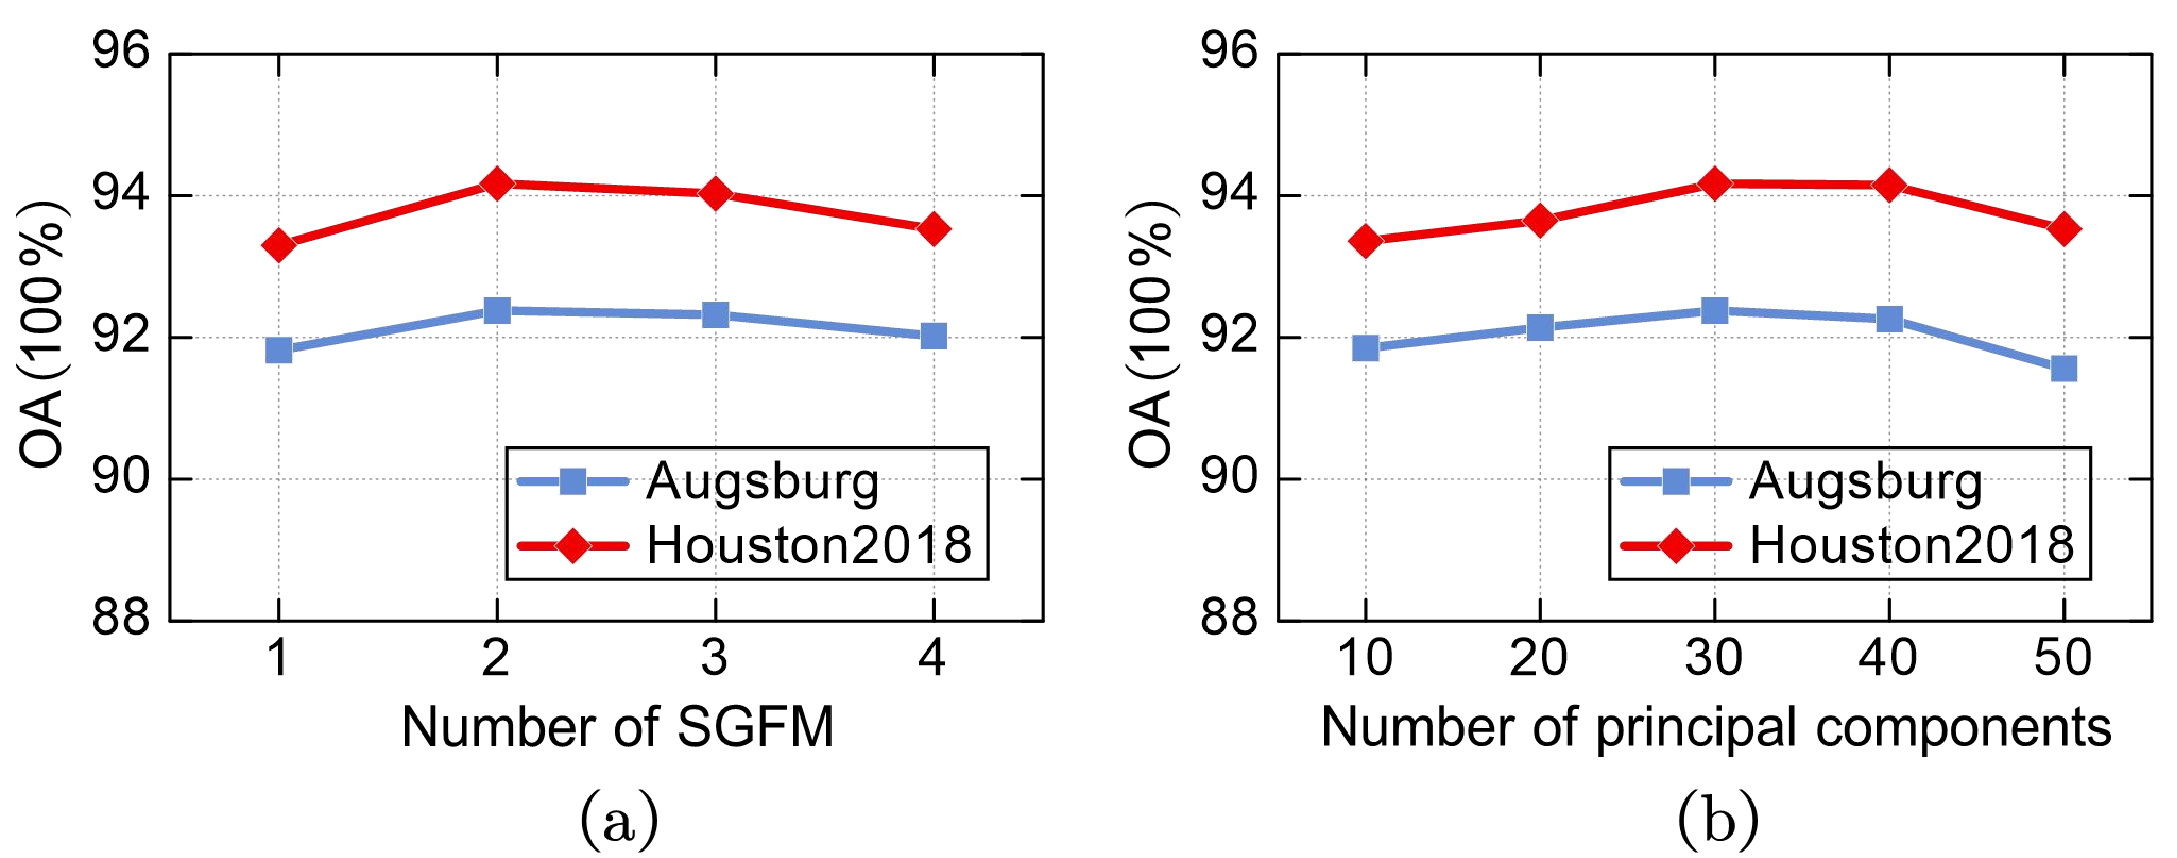
\includegraphics[width=3in]{figures/fig-para.pdf}
\caption{Parameter analysis. (a) The relationship between OA and the number of SGFM. (b) The relationship between OA and the number of principal components after PCA for HSI.}
  \label{fig_para}
\end{figure}

\textbf{Number of SGFM.} The number of SGFM is an important parameter that may affect the classification performance. We test different numbers of SGFM from 1 to 4. The experimental results are shown in Fig. \ref{fig_para}(a). When the number of SGFM is set to 2, our SGFNet achieves the best performance on both datasets. Therefore, in the following experiments, we use two SGFMs in the proposed SGFNet.

\textbf{Number of Principal Components for HSI.} HSI data contains rich spectral information but also introduces redundancy and spectral noise. Therefore, we use Principal Component Analysis (PCA) for HSI preprocessing. We tested the number of principal components for HSI, and the experimental results are shown in Fig. \ref{fig_para}(b). It can be observed that when the number of principal components is set to 30, our SGFNet achieves the best classification performance. Retaining too few components discards crucial discriminative spectral features, leading to suboptimal accuracy. Thus, the number of principal components is empirically set to 30.

\subsection{Experimental Results and Analysis}

\textbf{Results on the Augsburg Dataset.} Table \ref{table_augsburg} shows the quantitative evaluations on the Augsburg dataset. The OA value of the proposed SGFNet achieves 92.38\%, outperforming all the other methods. From the class-wise results, SGFNet achieves the best performance in the Industrial area and Allotment. Both categories usually exhibit complex spatial structures and significant spectral ambiguity, indicating that SGFNet can effectively capture discriminative semantic and contextual information.

\begin{table}
  \centering
  \caption{Experimental results on the Houston2018 dataset. The \textbf{bold} and \underline{underline} denote the best and second best results.}
  \setlength{\tabcolsep}{2pt} 
  \resizebox{0.9\linewidth}{!}{
  \begin{tabular}{c|cccccc}
  \hline\toprule
  Class                        & S$^2$ENet & DFINet & ExViT & DFFNet & MSFM & \cellcolor{bg} SGFNet \\
  \midrule
  Healthy grass                 & \textbf{99.15} & \underline{94.29} & 93.34 & 92.63 & 90.38 & \cellcolor{bg} 92.07 \\
  Stressed grass               & 84.35 & 92.71 & \underline{93.44} & 92.44 & \textbf{94.04} & \cellcolor{bg} 93.18 \\
  Artificial turf              & \textbf{100.0}   & \textbf{100.0}   & \textbf{100.0} & \textbf{100.0} & \textbf{100.0} & \cellcolor{bg} \textbf{100.0} \\
  Evergreen trees              & 98.13 & 98.92 & 95.87 & \underline{99.38} & 99.34 & \cellcolor{bg} \textbf{99.76} \\
  Deciduous trees              & 86.39 & 97.77 & 96.85 & \underline{99.16} & 99.11 & \cellcolor{bg} \textbf{99.94} \\
  Bare earth                   & 99.33 & \textbf{100.0}   & \textbf{100.0} & \underline{99.96} & \textbf{100.0} & \cellcolor{bg} \textbf{100.0} \\
  Water & \textbf{100.0}   & \textbf{100.0}   & \textbf{100.0} & \textbf{100.0} & \textbf{100.0} & \cellcolor{bg} \textbf{100.0} \\
  Residential buildings        & 97.17 & 97.36 & 97.39 & \underline{98.00} & 96.27 & \cellcolor{bg} \textbf{98.78} \\
  Non-residential buildings    & 93.93 & 93.29 & 93.00 & 93.73 & \underline{95.58} & \cellcolor{bg} \textbf{96.24} \\
  Roads                        & 70.17 & 75.73 & 72.18 & \underline{80.31} & 75.90 & \cellcolor{bg} \textbf{85.33} \\
  Sidewalks                    & 72.11 & \underline{83.67} & 69.69 & 72.59 & 81.43 & \cellcolor{bg} \textbf{84.64} \\
  Crosswalks                   & 82.47 & 94.23 & 88.12 & 91.84 & \underline{96.22} & \cellcolor{bg} \textbf{98.14} \\
  Major thoroughfares          & \textbf{89.44} & 81.20 & 86.12 & 84.54 & 86.89 & \cellcolor{bg} \underline{88.85} \\
  Highways                     & 98.53 & 98.91 & \textbf{99.50} & 98.82 & 98.63 & \cellcolor{bg} \underline{99.35} \\
  Railways                     & 99.21 & \textbf{99.94} & 99.87 & \underline{99.89} & 99.69 & \cellcolor{bg} 99.82 \\
  Paved parking lots           & 95.62 & 98.37 & 97.02 & 97.78 & \underline{98.94} & \cellcolor{bg}\textbf{99.34} \\
  Unpaved parking lots         & \textbf{100.0}   & \textbf{100.0}   & \textbf{100.0} & \textbf{100.0} & \textbf{100.0} & \cellcolor{bg}\textbf{100.0} \\
  Cars                         & 96.77 & \textbf{99.09} & 98.13 & \underline{98.89} & 97.81 & \cellcolor{bg}98.67 \\
  Trains                       & \textbf{100.0}   & 99.46 & \underline{99.98} & 99.91 & 99.97 & \cellcolor{bg}\textbf{100.0} \\
  Stadium seats                & \textbf{100.0}   & 99.98 & \underline{99.99} & \textbf{100.0} & \textbf{100.0} & \cellcolor{bg}\textbf{100.0} \\
  \midrule
  OA                           & 90.05 & 91.02 & 89.98 & 91.21 & \underline{92.38} & \cellcolor{bg}\textbf{94.17} \\
  AA                           & 93.14 & 95.24 & 94.02 & 94.99 & \underline{95.51} & \cellcolor{bg}\textbf{96.71} \\
  Kappa                        & 87.20 & 88.46 & 87.14 & 88.68 & \underline{90.16} & \cellcolor{bg}\textbf{92.46} \\
  \bottomrule\hline
  \end{tabular}}
  \label{table_houston2018}
\end{table}

\textbf{Results on the Houston2018 Dataset.} The classification maps on the Houston2018 dataset are shown in Fig. \ref{fig_results}, and the corresponding quantitative evaluations are illustrated in Table \ref{table_houston2018}. It can be observed that SGFNet produces classification maps that are more consistent with the ground truth, demonstrating superior land-cover discrimination capability. Table \ref{table_houston2018} shows that our SGFNet obtains the highest OA and Kappa, significantly outperforming other state-of-the-art methods. SGFNet achieves the best performance in several challenging categories, including Evergreen trees, Deciduous trees, Buildings, Roads, Sidewalks, Crosswalks, and Paved parking lots. These categories usually contain complex spatial distributions and strong spectral similarity with surrounding objects. The superior performance of SGFNet indicates that the proposed framework can effectively capture discriminative semantic information and exploit complementary features from multi-source data.

\begin{table}[!t]
\centering
\caption{Ablation study of the proposed SGFNet.}
\label{table_ablation}
\resizebox{0.65\linewidth}{!}{
\begin{tabular}{c|cc} 
\toprule
Model Variant & Augsburg & Houston2018 \\ 
\midrule
Baseline   & 88.54 & 89.65 \\
w/o SMCB   & 89.88 & 91.01 \\
w/o FMFB   & 91.29 & 92.37 \\ 
\rowcolor{bg}SGFNet (Full model) & \textbf{92.38} & \textbf{94.17} \\
\bottomrule
\end{tabular}}
\end{table}

\subsection{Ablation Study}

Table \ref{table_ablation} presents the ablation study results of the proposed SGFNet. The experiments are designed to evaluate the effectiveness of SMCB and FMFB. Starting from the baseline model, both modules consistently improve the classification performance. This demonstrates that SMCB can effectively enhance contextual representation capability, and FMFB effectively alleviates the slight spatial misalignment between multi-source data. The complete SGFNet achieves significant improvements of 3.84\% and 4.52\%, respectively. These results demonstrate that both proposed modules are complementary and jointly contribute to more robust multi-source feature fusion and classification.
